%%==================================================
%% chapter03.tex for SJTU Master Thesis
%% Encoding: UTF-8
%%==================================================

\chapter{应用重构上采样方法的流体动画基本框架}

本文第二章详细介绍了流体模拟的基本数学模型以及欧拉网格方法求解流体动画的基本计算框架,是本文研究的应用重构上采样方法的流体动画计算框架的基础知识。本章对欧拉网格方法的基本计算框架进行改进,提出了一个应用重构上采样方法的流体动画基本计算框架。

\section{流体动画疏密数据的特点}

低精度网格和高精度网格的流体场,都是由其局部细微结构组成,并且不同网格精度的流体场,其整体形态相似,只有局部细微结构不同。低精度网格流体场的信息量小于高精度网格流体场的信息量,我们需要一个经验上的数据集来弥补低-高精度流体场信息量上的差,表示两者之间的联系。而这个经验数据集,可通过学习大量的流体场数据获得。待解决的问题是,如何利用这个经验数据集来建立流体低-高精度样本之间的映射关系并加以利用?建立流体低-高精度样本之间的映射关系,并利用所建立的流体低-高精度样本之间的映射关系,就可以分解低精度流体场数据的稀疏表示,再映射到高精度流体场空间。进一步待解决的问题是,如何从低精度流体场快速映射到高精度流体场?如何建立高效的流体动画的重构上采样框架?

拟针对流体动画低-高精度流体场数据,由于数据之间有一定的相关性,满足了可压缩性信号的特点;而且整个流场数据常常存在零样本点,满足稀疏信号的定义。因此,流体场数据能满足压缩感知理论的信号稀疏的前提条件,适合运用基于压缩感知理论的方法进行稀疏重构上采样。为了建立一对经验上的数据集来表示流体动画低-高精度数据之间的关系,并将其利用到重构上采样方法中,本文收集大量的流体高精度网格上的速度场数据,并训练生成表示高精度网格速度场数据特征的训练字典,然后将该训练字典应用到流体动画低精度速度场数据与高精度速度场数据的重构上采样步骤中。本文的第四章将会详细介绍该代表低-高精度流体数据的映射关系的训练字典的方法以及将低精度流体场数据向高精度流体场映射的方法。

为了将过完备的训练字典技术应用到流体动画的疏密数据重构上采样框架中,并在尽可能少的时间耗费的情况下,尽可能多地模拟出高精度流体动画的细节,本文提出了一个基于欧拉网格模拟方法的流体动画重构上采样计算框架,本章的余下部分将会详细介绍该框架的内容。

\section{流体动画的重构上采样框架}

在流体动画领域,欧拉网格方法和拉格朗日粒子法都是比较常用的基本模拟方法。相较于欧拉网格方法,拉格朗日方法具有计算量小、模拟速度快等优点。但是在采样数据时,拉格朗日方法的数据来自于流体系统中大量运动的粒子,得到的每一帧流场数据为运动粒子在流体系统中对应位置上的点的数据,故不能保证每次都能在同一个位置上采样到流场数据。而欧拉方法的采样点对应于空间固定位置设置的大量网格点,故得到的每一帧流场数据为固定位置上的变量值。其采样特征不仅适用于实际采样点得到的数据,而且其数据结构形式适用于过完备稀疏字典重构上采样方法使用的数据结构。故本文使用欧拉网格方法作为流体动画模拟的基本框架。

欧拉网格法是流体动画领域最为常用的方法,该方法的模拟效果主要依赖于网格精度、对流方法的精度和投影操作收敛条件的大小,其中网格精度具有决定性的作用。当模拟精度提高一倍时,现有的精确模拟方法投影的计算耗时以 2 的 3 次方为倍数增长。针对欧拉方法提出的低-高精度重采样的优化方法的主要思想是将流体模拟过程中耗时最为显著的投影步骤放到低精度网格模拟,然后再使用上采样方法将低精度网格的流场数据映射到高精度网格。目前,该方法可以有效地加快流体动画模拟的速度,但是现有的方法都缺乏高效准确的重采样理论和方法的支持。为了能充分利用过完备训练字典重构上采样方法的特点,同时尽量减少投影步骤的耗时,本文借鉴低-高精度重采样方法,在投影步骤求解泊松方程之前, 将高精度的流体速度场数据投影到对应的低精度网格中,这样可以在低精度网格空间求解泊松方程。计算泊松方程,保证了流体的无散条件后,再利用过完备训练字典方法将低精度网格的流体速度场数据重构上采样到高精度空间,在高精度网格空间完成对流和加外力步骤。这样可以大大提高求解泊松方程的效率,进而整体上加速流体动画模拟的计算效率。图~\ref{simulationframework}给出了本文的基于过完备训练字典方法重构上采样的流体模拟基本框架。

\begin{figure}[ht]
  \centering
 \begin{tikzpicture}[
roundnode/.style={circle, draw=black, fill=lightgray!30, very thick, minimum size=2.4cm},
squarednode/.style={rectangle, draw=black, very thick},
]
%Nodes
\node[squarednode](upsample) at(5, 0) {\ \ \ \ \ \ \ \ \ 上采样\ \ \ \ \ \ \ \ \ \ \ };
\node[squarednode](boundary) at(0, 0) {\ \ \ \ \ \ \ 边界控制\ \ \ \ \ \ \ \ };
\node[squarednode](advect) at(0,1.5)  {\ \ \  对流(高精度)\ \ \ \ };
\node[squarednode](addForce) at(5,1.5)  {\ \ 加外力(高精度)\ \ };
\node[squarednode](downsample) at(10,1.5)  {\ \ \ \ \ \ \ \ 降采样\ \ \ \ \ \ \ \ \ \ };
\node[squarednode](project) at(10,0)  {\ \ \ 投影(低精度)\ \ \ };
%Lines
\draw[->, ultra thick] (advect) -- (addForce);
\draw[->, ultra thick] (addForce) -- (downsample);
\draw[->, ultra thick] (downsample) -- (project);
\draw[->, ultra thick] (project.west) -- (upsample);
\draw[->, ultra thick] (upsample) -- (boundary);
\draw[->, ultra thick] (boundary) -- (advect);
\end{tikzpicture}
%\caption{The simulation framework  based on up-sampling and reconstruction.}
\bicaption[fig:macgrid]{}{流体动画重构上采样框架}{Fig}{(a) The simulation framework  based on up-sampling and reconstruction}
\label {simulationframework}
\end{figure}

观察框架图~\ref{simulationframework}可以看出,本文方法的对流和加外力步骤都是在高精度网格完成的,只有高耗时的投影步骤是在低精度网格求解泊松方程的。因为计算对流步骤和加外力步骤的时间相较于投影步骤,可以忽略不计。但是在高精度网格空间计算对流步骤和投影步骤,能够获得更多的流体细节。而投影步骤在高精度网格上模拟,虽然也能产生大量的细节,但是时间开销过大。该框架旨在耗费尽量少的时间开销的情况下,尽可能多地模拟出流体的细节。

本章该部分的余下部分会详细介绍对流步骤和投影步骤的一般解决方案,流体速度场的降采样和重构上采样步骤将会在第四章进行详细介绍。

\subsection{对流}

流体基本步骤中的对流部分,求解的是在一个很短的时间间隔$\Delta t$内,流体沿其速度场对流一定距离后的各变量的变化。在计算机图形学领域,通常会根据对流部分的方程式的物理含义来求解该步骤。目前,针对对流操作已经提出了很多种高效的求解方法,并且对流过程的求解技术也已经趋于成熟。半拉格朗日方法是一种较为简单并且自提出后就被广泛使用的方法,为了提高半拉格朗日方法只有一阶精度的缺点,MacCormack方法对其进行了一些改进。半拉格朗日方法是求解对流步骤的基本方法,而MacCormack方法是后来针对半拉格朗日方法提出的改进方法的一种代表,在本文的实验中,我们主要应用了半拉格朗日方法和MacCormack方法实现对流,下面的内容将会简单介绍这两种方法的思想及实现。

\subsubsection{半拉格朗日方法}

拉格朗日方法将流体当作一个粒子系统来处理,半拉格朗日方法借鉴了拉格朗日方法的思想,从粒子的视角看待流体,但是同时也借鉴了欧拉方法的网格思想,通过后向追踪流体流过固定位置时的物理量更新当前位置物理量的值,故称该方法为半拉格朗日方法。图~\ref{fig:advection}给出了半拉格朗日方法后向追踪的示意图。图中变量$p(\boldsymbol x,t)$表示粒子随着时间的运行轨迹。

\begin{figure}[ht]
  \centering
   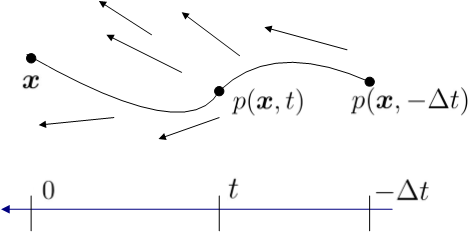
\includegraphics[height=1.7 in]{chap3/advection}
  \bicaption[fig:advection]{}{半拉格朗日对流方法示意图}{Fig}{Illustration of semi-Lagrangian advection method}
\end{figure}

根据图中所示,要求点$\boldsymbol x$处的速度场$\boldsymbol u$,后向追踪的思想是向后追踪一个时间间隔$\Delta t$,找到在$\Delta t$时间段前粒子的位置$p(\boldsymbol x, -\Delta t)$。根据欧拉网格方法的网格特性,已知粒子所处的位置,即获得其网格位置处存储的速度场等属性值。而又根据拉格朗日视角,对流步骤求解的方程式代表的含义是粒子携带的速度场是不会随着时间变化。故可以用粒子在$\Delta t$时间段前的速度场的旧值更新当前位置$\boldsymbol x$处的粒子的新值。但是,通过后向追踪计算得出的$\Delta t$时间段前粒子的位置$p(\boldsymbol x, -\Delta t)$有时会落在网格的边界以外,在这种情况下,我们采取的解决方案是简单地对点$\boldsymbol x$处的旧值做插值计算。下面的内容将会给出半拉格朗日方法的详细求解过程。

首先,我们设流体粒子当前的位置为$\boldsymbol x_{cur}$,在一个时间段$\Delta t$之前,它的位置为$\boldsymbol x_{pre}$,在半拉格朗日方法中,我们使用一步前向欧拉方法来估算时间段$\Delta t$之前粒子所处的位置$\boldsymbol x_{pre}$:
\begin{equation}
\boldsymbol x_{pre} = \boldsymbol x_{cur} - \Delta t \boldsymbol u_{cur}
\end{equation}

其中,$\boldsymbol u_{cur}$是流体在当前网格位置处的速度,因为粒子的速度不会随着时间的变化而变化,故此处我们可以用当前位置处的速度$\boldsymbol u_{cur}$前向追踪计算时间段$\Delta t$之前粒子所处的位置。

计算得到$\Delta t$之前粒子的位置$\boldsymbol x_{pre}$后,因为在大多数情况下,点$\boldsymbol x_{pre}$都不会落在网格区域内,故我们通常需要对临近网格的旧值$\boldsymbol u^n$做插值计算求得一个较好的近似值。此处我们设做插值计算的函数表示为$interpolate$,综上所述,可归纳出半拉格朗日方法的计算公式:
\begin{equation}
\boldsymbol u_{cur}^{n + 1} = interpolate({\boldsymbol u}^n, \boldsymbol x_{cur}  - \Delta t \boldsymbol u_{cur}^n)
\end{equation}

半拉格朗日方法是一种无条件稳定的数值算法,其算法具有简单易懂、可快速实现、计算高效等特点。Stam在1999年提出的半拉格朗日方法,树立了流体模拟基本方法的一个里程碑。但是该方法求解的结果只有一阶的数值精度,故存在较为严重的数值耗散问题。

\subsubsection{MacCormack方法}

MacCormack~\cite{maccormack2003effect}方法由MacCormack Robert提出,是一种双曲型偏微分方程的数值解法的解决方案。使用MacCormack方法求解欧拉网格方法的对流步骤,可分为两个部分,即后向追踪的预测步骤和前向追踪的修正步骤。其中,后向追踪的预测步骤与半拉格朗日方法的求解方案类似,为了克服半拉格朗日方法求解的结果只有一阶数值精度的缺点,MacCormack方法又提出了第二步前向追踪的修正步骤。对流体速度场进行修正之后的解决方案可以达到二阶数值精度,而在计算量上只增加了一个修正步骤,也就是计算开销也只有半拉格朗日方法的两倍。MacCormack方法能够模拟出比半拉格朗日对流方法多很多的细节,并且计算开销也不大,在流体动画领域被广为使用。

\begin{figure}
  \centering
   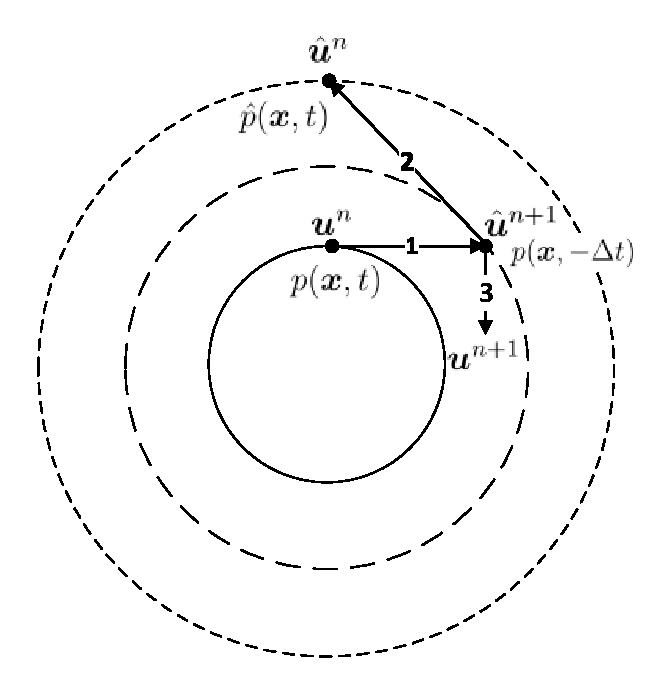
\includegraphics[height=2.5 in]{chap3/MacCormack}
  \bicaption[fig:MacCormack]{}{MacCormack对流方法示意图}{Fig}{Illustration of MacCormack advection method}
\end{figure}

图~\ref{fig:MacCormack}所示方法为Selle~\cite{selle2008unconditionally}在2007年提出的一种基于BFECC对流方法的无条件稳定的MacCormack方法。图中的带箭头的线段1表示向追踪的预测步骤。设半拉格朗日对流方法表示为$A(\boldsymbol u)$,
该步骤对位于当前位置点$p(\boldsymbol x,t)$处的粒子的速度场$\boldsymbol u^n$做一次对流计算,可计算得出点$p(\boldsymbol x, -\Delta t)$处的粒子在时间段$\Delta t$之前的速度$\boldsymbol {\hat u}^{n + 1}$如下方程式所示:
\begin{equation}
\boldsymbol {\hat u}^{n + 1}  = A(\boldsymbol u^n)
\end{equation}

修正步骤在图~\ref{fig:MacCormack}中表示为线段2和线段3。观察线段2,可知该步骤表示的含义是以时间段$\Delta t$之前的粒子的速度场和位置$p(\boldsymbol x, -\Delta t)$为起点,前向追踪$\Delta t$时间段之后粒子所在的位置$\hat p(\boldsymbol x,t)$。与半拉格朗日方法类似,此处计算生成的粒子所处的位置$\hat p(\boldsymbol x,t)$往往也不会落在网格区域内,故我们也需要对其进行插值计算,才能生成该位置处的速度$\hat {\boldsymbol u}^n$。设第二步前向追踪与插值的结果表示为$A^R(\boldsymbol u)$,那么修正步骤的方程式可以表示为:
\begin{equation}
\boldsymbol {\hat u}^{n}  = A^R(\boldsymbol u^{n + 1})
\end{equation}

由步骤2计算出的粒子所处的位置$\hat p(\boldsymbol x,t)$为估算的粒子当前位置,可认为其与粒子当前所处的实际位置之间的差值$p(\boldsymbol x,t)$为第一步后向追踪步骤的计算误差,表示成$e = (\hat {\boldsymbol u}^n - \boldsymbol u^n) / 2$,那么当前位置$p(\boldsymbol x,t)$处的速度场可由下列式子计算得出:
\begin{equation}
\boldsymbol {u}^{n + 1}  = A(\boldsymbol u^n) - e = \hat {\boldsymbol u}^{n + 1} - e
\end{equation}

对上述式子做整理变换,最后可得更新速度场$\boldsymbol u^{n + 1}$的计算公式如下所示:
\begin{equation}
\label{eq:MacCormack}
\boldsymbol {u}^{n + 1}  = \hat {\boldsymbol u}^{n + 1} + (\boldsymbol u^n - \hat {\boldsymbol u}^n) / 2
\end{equation}

\subsection {投影}

观察第二章对流方程式~\ref{eq:advection}和加外力方程式~\ref{eq:addForce},可以看出这两项的计算不能保证流体的不可压缩条件。故我们需要一个额外的步骤,将对流和加外力后的速度场投影到无散空间,而投影步骤实现的就是速度场数据的无散约束条件。但是,观察方程式~\ref{eq:projection},可以看出该方程式的求解不仅包含未知量速度场$\boldsymbol u$,还包含未知量压强场$p$,相较于对流和加外力步骤,投影步骤的求解过程要复杂很多。

首先,我们需要在2D场景下的MAC网格中对速度场做离散化,根据方程式~\ref{eq:projection}的压力项公式,可以得到下面的速度场离散形式:
\begin{equation}
\label{eq:pressureu}
u_{i + 1 / 2, j}^{n + 1} = u_{i + 1 / 2, j}^n - \Delta \frac{1}{\rho} \frac{p_{i + 1, j} - p_{i, j}}{\Delta x}
\end{equation}
\begin{equation}
\label{eq:pressurev}
v_{i + 1 / 2, j}^{n + 1} = v_{i, j +1 / 2}^n - \Delta \frac{1}{\rho} \frac{p_{i, j + 1} - p_{i, j}}{\Delta x}
\end{equation}

其中,$\Delta x$表示MAC网格单元的宽度。观察方程式~\ref{eq:pressureu}~和方程式\ref{eq:pressurev},我们知更新速度场,需要先计算出包含流体的网格单元中心位置处的压强场。

另外,我们还可以根据方程式~\ref{eq:projection}的不可压缩条件推导的公式离散流体的速度场。在2D场景下的MAC网格中根据不可压缩条件离散化流体的速度场,有如下表示形式:
\begin{equation}
\label{eq:imcompressibleMAC}
\frac{u_{i + 1 / 2, j}^{n + 1} - u_{i - 1 / 2, j}^{n + 1}}{\Delta x} + 
\frac{v_{i, j + 1 / 2}^{n + 1} - v_{i, j - 1 / 2}^{n + 1}}{\Delta x}
= 0
\end{equation}

将上述方程~\ref{eq:pressureu}和~\ref{eq:pressurev}代入到方程式~\ref{eq:imcompressibleMAC}中,并对其进行整理合并,我们有:
\begin{multline}
\label{eq:impAndpress}
\frac{\Delta t}{\rho} (\frac{4p_{i,j} - p_{i + 1,j} - p_{i, j + 1} - p_{i - 1, j} - p_{i,j - 1}}{\Delta x^2}) \\
= - (\frac{u_{i + 1 / 2, j}^n - u_{i - 1 / 2, j}^n}{\Delta x} +
 \frac{v_{i, j + 1 / 2}^n - v_{i, j - 1/2}^n}{\Delta x})
\end{multline}

观察方程式~\ref{eq:impAndpress},可以看出其在表现形式上近似于泊松问题方程式$-\Delta t / \rho \nabla\ \cdot \nabla p = - \nabla \cdot \boldsymbol u$。

但是,直接只用上述方程式,只能处理流体内部速度场数据的无散条件。而在流体模拟的实际应用场景中,往往会存在多种类型的边界条件,如在流体内部运动的物体与流体的边界、流体的自由表面(尤其是水与空气的接触面)以及流体的包围边界等。当考虑到边界条件时,即将上述方程式应用到流体的边界区域时,需要区分压强的不同边界条件。在此处为了方便讨论,我们可以简单地将网格单元分成流体单元、固体单元或者气体单元,更复杂的分类模型需要增加部分包含流体或部分包含气体等的单元分类,但是在本章节的讨论中,我们暂不考虑。

%%%%%%%%%%%%%%%%%%%%%%%%%%%%%%
\begin{figure}[ht]
  \centering
   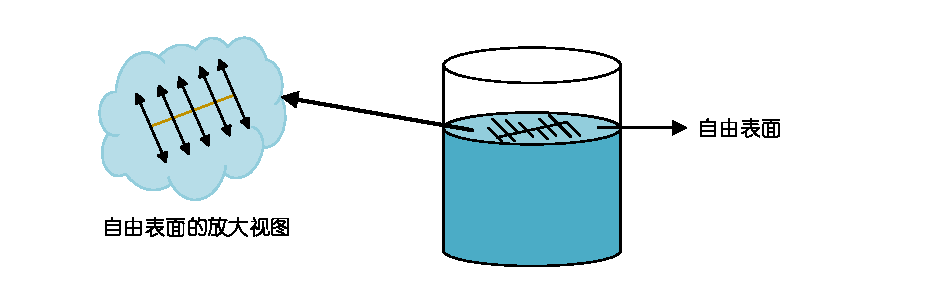
\includegraphics[height=1.9 in]{chap3/free_surface}
  \bicaption[fig:freeSurface]{}{水的自由表面示意图}{Fig}{Illustration of free-surface of liquid}
\end{figure}
%%%%%%%%%%%%%%%%%%%%%%%%%%%%%%%

在水动画的模拟计算中,自由表面边界是一类相对简单的边界条件,如图~\ref{fig:freeSurface}所示。通常,我们使用一种很简单的方法来标记这种边界条件,即将流体外部的网格单元的压强全部设置为0,我们称这样的边界为Dirichlet边界。

更复杂一点的边界是固体边界。这种边界条件有多种情况,如在液体内部运动或者静止的物体表面与液体接触的部分等。在这些边界处,设存储的速度分量为$\boldsymbol u \cdot \hat {\boldsymbol n}$,其中,变量$\hat {\boldsymbol n}$表示单位法向量。这样的边界在求压强梯度时,需要保证边界条件$\boldsymbol u^{n + 1} \cdot \hat {\boldsymbol n}$。通常,称这样的边界为Neumann边界条件。假设网格单元$(i, j)$表示流体单元,而网格单元$(i + 1, j)$表示固体单元,那么速度$u_{i + 1 / 2, j}$可以用下面的方程式更新:
\begin{equation}
u_{i + 1 / 2, j} ^{n + 1} = u_{i + 1 / 2, j}^n - 
\Delta t \frac{1}{\rho} \frac{p_{i + 1, j} - p _{i, j}}{\Delta x}
\end{equation}

因为$u_{i + 1 / 2, j} ^{n + 1}$是固体单元,故可用固体运动的速度变量$u_{neumann\_solid}$表示。将Neumann边界条件代入到方程式~\ref{eq:impAndpress}中,可得:
\begin{equation}
\frac{\Delta t}{\rho}\frac{3p_{i, j} - p_{i - 1, j} - p_{i, j - 1}}{\Delta x^2} = -(\frac{u_{neumann\_solid} - u_{i - 1 / 2, j}^{n}}{\Delta x}  +
\frac{v_{i, j + 1 / 2}^n - v_{i, j - 1 / 2}^n}{\Delta x})
\end{equation}

对上述方程式进行整理,有:
\begin{equation}
\label{eq:proj}
{3p_{i, j} - p_{i - 1, j} - p_{i, j - 1}}= -\frac{\rho \Delta x}{\Delta t}({u_{neumann\_solid} - u_{i - 1 / 2, j}^{n}}  +
{v_{i, j + 1 / 2}^n - v_{i, j - 1 / 2}^n})
\end{equation}

在逐帧迭代求解上述方程式的过程中,当前帧的速度场$\boldsymbol u^n$和Neumann边界速度$u_{neumann\_solid}$均可当作已知值,观察上式可以看出,该方程式只有一个未知压强变量场$p$,故我们可以通过上述方程式求解MAC网格中心位置的压强场,计算得出压强场后,即可根据方程式~\ref{eq:pressureu}求出流体下一帧的速度场。

在流体模拟领域,通常会将方程式~\ref{eq:proj}转换成相应的矩阵的形式:
\begin{equation}
\label{eq:matrixform}
\boldsymbol {Ap} = \boldsymbol {d}
\end{equation}

 其中,$A$是一个对称正定的稀疏矩阵,与网格中的边界的分布相关。$\boldsymbol p$是压强场,$\boldsymbol d$表示方程式~\ref{eq:proj}的右边部分。观察求解压强场的矩阵方程式可以看出,该方程式为一个线性方程式,并且形式十分简单,可以直接求解。但是,在流体模拟的计算中,由于网格精度比较高,导致矩阵A往往很大,从而使得方程式~\ref{eq:matrixform}的计算开销也很大。事实上,投影步骤的高耗时也是因为求解式~\ref{eq:matrixform}造成的。目前,已经出现了一批成熟的求解上述方程式的算法,如传统的PCG(Preconditioned Conjugate Gradient ) solver以及由PCG扩展出的Multigrid PCG~\cite{mcadams2010parallel}、ICPCG等,这些方法可以较为高效地模拟求解投影步骤,但是针对大规模的流体动画,其时间耗费还是非常大。

\section{本章小结}

本章结合流体动画低高精度流体场数据的特点,提出了本文的应用低-高精度流体场数据重采样步骤的流体动画计算框架,并详细介绍了该计算框架的对流步骤和投影步骤。本章还详细介绍了半拉格朗日对流方法和MacCormack对流方法,并指出半拉格朗日方法存在求解精度只能达到一阶的问题,MacCormack方法是对半拉格朗日方法的改进,在只提高一倍计算开销的前提下,达到二阶的精度的数值解。

在本文提出的流体动画基本框架中,对流步骤和加外力步骤在高精度网格中计算,只有投影步骤是在低精度网格中求解的,这样可以有效地减少投影步骤的计算开销,而又不丢失对流和加外力步骤求解结果的数值精度。


